\begin{name}
	{\tenchude}
	{\tendethi}
	{LỚP TOÁN THẦY PHÁT}
	{\lq\lq  It's not how much time you have, it's how you use it.\rq\rq}
\end{name}

\Opensolutionfile{ans}[ans/De-TB-Yeu-So-1]
\TN
\begin{ex}%[2D4H1-2]
	Tìm $\displaystyle\int (2x-3)\mathrm{\,d}x$.
	\choice
	{$x^2+C$}
	{$x^2-3x$}
	{\True $x^2-3x+C$}
	{$2x^2+3x+C$}
	\loigiai{
		Ta có áp dụng các tính chất cơ bản của nguyên hàm
		\begin{eqnarray*}
\displaystyle\int (2x-3)\mathrm{\,d}x&=&\displaystyle\int 2x\mathrm{\,d}x-\displaystyle\int 3\mathrm{\,d}x\\&=&2\cdot \dfrac{x^2}{2}-3x+C\\&=&x^2-3x+C.
\end{eqnarray*}
		Vậy nguyên hàm của hàm số đã cho là $x^2-3x+C$.
	}
\end{ex}

\begin{ex}%[1D1H5-3]
	Nghiệm phương trình $\sin 2x=-\dfrac{\sqrt{2}}{2}$ là
	\choice
	{\True $\hoac{&x=-\dfrac{\pi}{8}+k\pi\\&x=\dfrac{5\pi}{8}+k\pi}$}
	{$\hoac{&x=\dfrac{\pi}{4}+k\pi\\&x=\dfrac{3\pi}{4}+k\pi}$}
	{$\hoac{&x=\dfrac{\pi}{8}+k\pi\\&x=\dfrac{3\pi}{8}+k\pi}$}
	{$\hoac{&x=\dfrac{\pi}{4}+k2\pi\\&x=\dfrac{3\pi}{4}+k2\pi}$}
	\loigiai{
		Ta có
		\begin{eqnarray*}
&&\sin 2x=-\dfrac{\sqrt{2}}{2}\\&\Leftrightarrow &\sin 2x=\sin \left(-\dfrac{\pi}{4}\right)\\&\Leftrightarrow &\hoac{&2x=-\dfrac{\pi}{4}+k2\pi\\&2x=\pi-\left(-\dfrac{\pi}{4}\right)+k2\pi}\\&\Leftrightarrow &\hoac{&2x=-\dfrac{\pi}{4}+k2\pi\\&2x=\dfrac{5\pi}{4}+k2\pi}\\&\Leftrightarrow &\hoac{&x=-\dfrac{\pi}{8}+k\pi\\&x=\dfrac{5\pi}{8}+k\pi}\quad(k\in \mathbb{Z}).
\end{eqnarray*}
		Vậy nghiệm của phương trình là $\hoac{&x=-\dfrac{\pi}{8}+k\pi\\&x=\dfrac{5\pi}{8}+k\pi}$ $(k\in \mathbb{Z})$.
	}
\end{ex}

\begin{ex}%[2D1H3-1]
	Tìm giá trị lớn nhất $M$ của hàm số $y=\dfrac{3x-1}{x-3}$ trên đoạn $[0;2]$.
	\choice
	{$M=-5$}
	{\True $M=\dfrac{1}{3}$}
	{$M=-\dfrac{1}{3}$}
	{$M=5$}
	\loigiai{
		Điều kiện xác định $x\neq3$.\\
		Vì $3\notin[0;2]$ nên hàm số $y=\dfrac{3x-1}{x-3}$ xác định và liên tục trên đoạn $[0;2]$.\\
		Ta có $y'=\dfrac{3\cdot (-3)-1\cdot (-1)}{(x-3)^2}=-\dfrac{8}{(x-3)^2}$.\\
		Ta thấy $y'<0$, $\forall x\in [0;2]$, do đó hàm số nghịch biến trên đoạn $[0;2]$.\\
		Suy ra giá trị lớn nhất của hàm số trên đoạn $[0;2]$ đạt được tại $x=0$.\\
		Ta có $y(0)=\dfrac{3\cdot 0-1}{0-3}=\dfrac{1}{3}$ và $y(2)=\dfrac{3\cdot 2-1}{2-3}=-5$.\\
		Vậy giá trị lớn nhất của hàm số là $M=\max \limits_{[0;2]}y=y(0)=\dfrac{1}{3}$.
	}
\end{ex}

\begin{ex}%[1D6H4-2]
	Nghiệm của phương trình $\log _{16}(x+5)=\dfrac{1}{2}$ là
	\choice
	{\True $-1$}
	{$27$}
	{$3$}
	{-$3$}
	\loigiai{
		Điều kiện xác định $x+5>0\Leftrightarrow x>-5$.\\
		Phương trình đã cho tương đương với
		\begin{eqnarray*}
&&x+5=16^{\tfrac{1}{2}}\\&\Leftrightarrow &x+5=\sqrt{16}\\&\Leftrightarrow &x+5=4\\&\Leftrightarrow &x=-1\text{ (thỏa mãn điều kiện)}.
\end{eqnarray*}
		Vậy nghiệm của phương trình là $x=-1$.
	}
\end{ex}

\begin{ex}%[2H5N3-2]
	Trong không gian $Oxyz$, cho mặt cầu $(S)\colon (x+2)^2+(y+1)^2+z^2=81$. Tìm tọa độ tâm $I$ và tính bán kính $R$ của mặt cầu $(S)$.
	\choice
	{$I(2;1;0)$, $R=81$}
	{\True $I(-2;-1;0)$, $R=9$}
	{$I(2;1;0)$, $R=9$}
	{$I(-2;-1;0)$, $R=81$}
	\loigiai{
		Phương trình mặt cầu dạng chuẩn là $(x-a)^2+(y-b)^2+(z-c)^2=R^2$, trong đó tâm là $I(a;b;c)$ và bán kính là $R>0$.\\
		Biến đổi phương trình mặt cầu $(S)$ đã cho về dạng chuẩn, ta được
		\begin{align*}
\left[x-(-2)\right]^2+\left[y-(-1)\right]^2+(z-0)^2=9^2.
\end{align*}
		Đồng nhất hệ số, ta suy ra mặt cầu $(S)$ có tâm $I(-2;-1;0)$ và bán kính $R=\sqrt{81}=9$.\\
		Vậy tọa độ tâm $I(-2;-1;0)$ và bán kính $R=9$.
	}
\end{ex}

\begin{ex}%[2D4N2-1]
	Cho hai hàm số $f(x)$ và $g(x)$ liên tục trên $K$, $a$, $b\in K$. Khẳng định nào sau đây là khẳng định \textbf{sai}?
	\choice
	{$\displaystyle\int \limits_a^b\left[f(x)+g(x)\right]\mathrm{\,d}x=\displaystyle\int \limits_a^bf(x)\mathrm{\,d}x+\displaystyle\int \limits_a^bg(x)\mathrm{\,d}x$}
	{$\displaystyle\int \limits_a^bkf(x)\mathrm{\,d}x=k\displaystyle\int \limits_a^bf(x)\mathrm{\,d}x$}
	{$\displaystyle\int \limits_a^b\left[f(x)-g(x)\right]\mathrm{\,d}x=\displaystyle\int \limits_a^bf(x)\mathrm{\,d}x-\displaystyle\int \limits_a^bg(x)\mathrm{\,d}x$}
	{\True $\displaystyle\int \limits_a^bf(x)g(x)\mathrm{\,d}x=\displaystyle\int \limits_a^bf(x)\mathrm{\,d}x\cdot \displaystyle\int \limits_a^bg(x)\mathrm{\,d}x$}
	\loigiai{
		Theo các tính chất cơ bản của tích phân xác định đối với các hàm số liên tục, ta có
		\begin{itemize}
			\item Tích phân của một tổng/hiệu bằng tổng/hiệu các tích phân. Do đó hai khẳng định chứa phép cộng và phép trừ là đúng.
			\item Có thể đưa hằng số $k$ ra ngoài dấu tích phân. Do đó khẳng định chứa phép nhân với hằng số là đúng.
			\item Tích phân \textbf{không} có tính chất phân phối đối với phép nhân hai hàm số (tích phân của một tích nói chung không bằng tích các tích phân).
		\end{itemize}
		Vậy khẳng định $\displaystyle\int \limits_a^bf(x)g(x)\mathrm{\,d}x=\displaystyle\int \limits_a^bf(x)\mathrm{\,d}x\cdot \displaystyle\int \limits_a^bg(x)\mathrm{\,d}x$ là khẳng định sai.
	}
\end{ex}

\begin{ex}%[2D6H1-2]
	Cho hai biến cố độc lập $A$, $B$ với $\mathrm{P}(A)=0{,}6$, $\mathrm{P}(B)=0{,}45$. Khi đó, $\mathrm{P}(B\mid A)$ bằng
	\choice
	{$0{,}15$}
	{\True $0{,}45$}
	{$0{,}75$}
	{$0{,}6$}
	\loigiai{
		Theo định nghĩa, hai biến cố $A$ và $B$ được gọi là độc lập nếu việc xảy ra hay không xảy ra của biến cố này không làm ảnh hưởng tới xác suất xảy ra của biến cố kia.\\
		Nói cách khác, xác suất có điều kiện của $B$ khi biết $A$ đã xảy ra chính bằng xác suất của $B$.\\
		Do $A$ và $B$ độc lập nên ta có $\mathrm{P}(B\mid A)=\mathrm{P}(B)$.\\
		Theo giả thiết ta có $\mathrm{P}(B)=0{,}45$, suy ra $\mathrm{P}(B\mid A)=0{,}45$.\\
		Vậy $\mathrm{P}(B\mid A)=0{,}45$.
	}
\end{ex}

\begin{ex}%[1H8H6-1]
	Cho hình chóp $S.ABC$ có $SA\perp (ABC)$. Góc giữa $SC$ và mặt phẳng $(ABC)$ là góc nào trong các góc sau?
	\choice
	{$\widehat{BSC}$}
	{$\widehat{SCB}$}
	{$\widehat{ASC}$}
	{\True $\widehat{SCA}$}
	\loigiai{
		Ta có $SA\perp (ABC)$ nên hình chiếu vuông góc của đỉnh $S$ lên mặt phẳng $(ABC)$ là điểm $A$.\\
		Lại có điểm $C$ nằm trên mặt phẳng $(ABC)$ nên hình chiếu của chính nó là $C$.\\
		Suy ra đoạn thẳng $AC$ là hình chiếu vuông góc của đoạn thẳng $SC$ lên mặt phẳng $(ABC)$.\\
		Góc giữa đường thẳng và mặt phẳng là góc giữa đường thẳng đó và hình chiếu của nó trên mặt phẳng. Do đó, góc giữa $SC$ và mặt phẳng $(ABC)$ là góc giữa $SC$ và $AC$.\\
		Vì tam giác $SAC$ vuông tại $A$ nên góc giữa hai đường thẳng $SC$ và $AC$ chính là góc nhọn $\widehat{SCA}$.\\
		Vậy góc cần tìm là $\widehat{SCA}$.
	}
\end{ex}

\begin{ex}%[2D1N1-2]
	Cho hàm số $y=f(x)$ có bảng biến thiên như sau
	\begin{center}
		
\begin{tikzpicture}
			\tkzTabInit[nocadre=false,lgt=1,espcl=2.5,deltacl=0.5]
			{$x$/0.6,$y'$/0.6,$y$/2.5}
			{$-\infty$,$0$,$2$,$+\infty$}
			\tkzTabLine{,+,0,-,0,+}
			\tkzTabVar{-/$-\infty$,+/$1$,-/$3$,+/$+\infty$}
		\end{tikzpicture}
	\end{center}
	Hàm số đã cho đồng biến trên khoảng nào dưới đây?
	\choice
	{$(-\infty;1)$}
	{$(0;2)$}
	{$(0;+\infty)$}
	{\True $(2;+\infty)$}
	\loigiai{
		Hàm số đồng biến trên các khoảng mà tại đó đạo hàm $y'>0$.\\
		Dựa vào bảng biến thiên, ta thấy $y'>0$ trên hai khoảng là $(-\infty;0)$ và $(2;+\infty)$.\\
		Đối chiếu với các đáp án đã cho, ta thấy khoảng $(2;+\infty)$ là một khoảng đồng biến của hàm số.\\
		Vậy hàm số đồng biến trên khoảng $(2;+\infty)$.
	}
\end{ex}

\begin{ex}%[1D2N2-2]
	Trong các dãy số sau, dãy số nào là một cấp số cộng?
	\choice
	{$1$; $-3$; $-6$; $-9$; $-12$}
	{$1$; $-2$; $-4$; $-6$; $-8$}
	{$1$; $-3$; $-5$; $-7$; $-9$}
	{\True $1$; $-3$; $-7$; $-11$; $-15$}
	\loigiai{
		Dãy số $(u_n)$ là một cấp số cộng nếu hiệu của hai số hạng liên tiếp luôn là một hằng số $d$ (gọi là công sai), tức là $u_{n+1}-u_n=d$, $\forall n\geq 1$.\\
		Ta tiến hành kiểm tra hiệu các số hạng liên tiếp của từng đáp án
		\begin{itemize}
			\item Dãy $1$; $-3$; $-6$; $-9$; $-12$ có $(-3)-1=-4$, nhưng $(-6)-(-3)=-3\neq-4$ (loại).
			\item Dãy $1$; $-2$; $-4$; $-6$; $-8$ có $(-2)-1=-3$, nhưng $(-4)-(-2)=-2\neq-3$ (loại).
			\item Dãy $1$; $-3$; $-5$; $-7$; $-9$ có $(-3)-1=-4$, nhưng $(-5)-(-3)=-2\neq-4$ (loại).
			\item Dãy $1$; $-3$; $-7$; $-11$; $-15$ có: $(-3)-1=(-7)-(-3)=(-11)-(-7)=(-15)-(-11)=-4$ (thỏa mãn).
		\end{itemize}
		Vậy dãy số $1$; $-3$; $-7$; $-11$; $-15$ là một cấp số cộng với số hạng đầu $u_1=1$ và công sai $d=-4$.
	}
\end{ex}

\begin{ex}%[1D5N2-2]
	Trung vị của mẫu số liệu ghép nhóm
	\choice
	{là giá trị xấp xỉ cho mẫu số liệu gốc và không thể lấy làm giá trị đại diện cho mẫu số liệu}
	{chia mẫu số liệu đã sắp xếp theo thứ tự không giảm thành bốn phần bằng nhau}
	{\True là giá trị xấp xỉ cho mẫu số liệu gốc và có thể lấy làm giá trị đại diện cho mẫu số liệu}
	{xác định chính xác trung vị của mẫu số liệu gốc}
	\loigiai{
		Trung vị của mẫu số liệu ghép nhóm là giá trị xấp xỉ cho mẫu số liệu gốc và có thể lấy làm giá trị đại diện cho mẫu số liệu.
	}
\end{ex}

\begin{ex}%[1D6H3-1]
	Cho $a$ là số thực dương khác $1$. Mệnh đề nào dưới đây \textbf{sai}?
	\choice
	{$\log _{a}a^2=2$}
	{$3^{\log _3a}=a$}
	{$a^{-\log _a2}=\dfrac{1}{2}$}
	{\True $\log _{a^3}a=3$}
	\loigiai{
		Với $a>0$ và $a\neq1$, ta áp dụng các tính chất cơ bản của lôgarit để kiểm tra từng mệnh đề:
		\begin{itemize}
			\item $\log _{a}a^2=2\log _aa=2\cdot 1=2\Rightarrow$ đúng.
			\item Sử dụng công thức $a^{\log _ab}=b$, ta có $3^{\log _3a}=a\Rightarrow$ đúng.
			\item $a^{-\log _a2}=a^{\log _a2^{-1}}=2^{-1}=\dfrac{1}{2}\Rightarrow$ đúng.
			\item $\log _{a^3}a=\dfrac{1}{3}\log _aa=\dfrac{1}{3}\cdot 1=\dfrac{1}{3}\neq3\Rightarrow$ sai.
		\end{itemize}
		Vậy mệnh đề sai là $\log _{a^3}a=3$.
	}
\end{ex}

\cauds
\begin{ex}%[1D7H1-4]
	Một chất điểm chuyển động có phương trình $s(t)$ thì có vận tốc $v(t)=s'(t)$. Biết rằng phương trình chuyển động của chất điểm là $s(t)=\dfrac{1}{3}t^3-3t^2+5t$ trong đó $t$ được tính bằng giây và $s$ được tính bằng mét.
	\choiceTF
	{\True Vận tốc của chất điểm tại thời điểm $t$ được tính bởi $v(t)=t^2-6t+5$}
	{\True Gia tốc của chất điểm tại thời điểm $t=2$ là $a(2)=-2$ (m/s$^2$)}
	{Trong $5$ giây đầu tiên, vận tốc của chất điểm luôn giảm dần}
	{\True Kể từ giây thứ $3$ trở đi thì vận tốc của chất điểm bắt đầu tăng}
	\loigiai{
		\begin{itemchoice}
			\itemch Ta có vận tốc $v(t)=s'(t)=\left(\dfrac{1}{3}t^3-3t^2+5t\right)'=t^2-6t+5$.
			\itemch Gia tốc của chất điểm là $a(t)=v'(t)=2t-6$.\\
			Tại thời điểm $t=2\Rightarrow a(2)=2\cdot 2-6=-2$ (m/s$^2$).
			\itemch Xét trên khoảng thời gian $5$ giây đầu tiên $t\in (0;5)$:\\
			Ta có $a(t)=0\Leftrightarrow 2t-6=0\Leftrightarrow t=3$.\\
			Ta thấy $a(t)<0$ khi $t\in (0;3)$ và $a(t)>0$ khi $t\in (3;5)$.\\
			Do đó, vận tốc của chất điểm giảm trên khoảng $(0;3)$ và tăng trên khoảng $(3;5)$.
			\itemch Theo phân tích ở trên, vận tốc tăng khi gia tốc $a(t)>0\Leftrightarrow t>3$. \\
			Do đó kể từ giây thứ $3$ trở đi thì vận tốc của chất điểm bắt đầu tăng.
		\end{itemchoice}
	}
\end{ex}

\begin{ex}%[2H5V3-2]
	Trong không gian với hệ trục toạ độ $Oxyz$, cho mặt cầu có phương trình $(S)\colon x^2+y^2+z^2+2x-4y-6z+m-3=0$ và mặt phẳng $(\beta)\colon 2x-y+2z-8=0$.
	\choiceTF
	{$(S)\colon x^2+y^2+z^2+2x-4y-6z+m-3=0$ là phương trình mặt cầu khi và chỉ khi $m\leq 17$}
	{\True Mặt phẳng $(\beta)$ có vectơ pháp tuyến là $\overrightarrow{n}=(2;-1;2)$}
	{Có hai số thực của tham số $m$ để mặt phẳng $(\beta)\colon 2x-y+2z-8=0$ cắt $(S)$ theo một đường tròn có chu vi bằng $8\pi$}
	{\True Khoảng cách từ tâm của mặt cầu $(S)$ đến $(\beta)$ là $2$}
	\loigiai{
		\begin{itemchoice}
			\itemch Ta có $(S)\colon x^2+y^2+z^2+2x-4y-6z+m-3=0\Leftrightarrow (x+1)^2+(y-2)^2+(z-3)^2=17-m$.\\
			Để $(S)$ là phương trình của một mặt cầu thì $R^2=17-m>0\Leftrightarrow m<17$.
			\itemch Từ phương trình mặt phẳng $(\beta)\colon 2x-y+2z-8=0$, ta dễ dàng suy ra vectơ pháp tuyến là $\overrightarrow{n}=(2;-1;2)$.
			\itemch Mặt cầu $(S)$ có tâm $I(-1;2;3)$ và bán kính $R=\sqrt{17-m}$ (với $m<17$).\\
			Để đường tròn giao tuyến có chu vi bằng $8\pi$ thì bán kính $r$ của đường tròn đó là \[2\pi r=8\pi\Leftrightarrow r=4.\]
			Khoảng cách từ tâm $I$ đến $(\beta)$ là $d=\dfrac{|2\cdot (-1)-2+2\cdot 3-8|}{\sqrt{2^2+(-1)^2+2^2}}=\dfrac{6}{3}=2$.\\
			Theo định lý Pytago ta có $R^2=\mathrm{d}^2+r^2\Leftrightarrow 17-m=2^2+4^2\Leftrightarrow 17-m=20\Leftrightarrow m=-3$.
			\itemch Dựa vào quá trình tính toán ở ý trên, khoảng cách từ tâm mặt cầu $(S)$ đến $(\beta)$ là $\mathrm{d}\big(I,(\beta)\big)=2$.
		\end{itemchoice}
	}
\end{ex}

\begin{ex}%[2D4H1-6]
	Trong $5$ giây đầu tiên, một chất điểm chuyển động với vận tốc $v(t)=-3t^2+12t+1$ (m/s), $s(t)$ là quãng đường chuyển động của chất điểm theo thời gian $t$.
	\choiceTF
	{Trong $5$ giây đầu tiên, vận tốc lớn nhất của chất điểm là $3$ (m/s)}
	{\True Quãng đường chuyển động của chất điểm trong $5$ giây đầu tiên là $30$ (m)}
	{Vận tốc của vật tại thời điểm $t=2$ là $v(2)=1$ (m/s)}
	{\True Trong khoảng thời gian từ $t=2$ đến $t=5$ vận tốc của chất điểm giảm dần}
	\loigiai{
		\begin{itemchoice}
			\itemch Ta có $v'(t)=-6t+12$; $v'(t)=0\Leftrightarrow t=2\in [0;5]$.\\
			Tính các giá trị vận tốc tại các điểm cực trị và đầu mút là $v(0)=1$, $v(2)=13$, $v(5)=-14$.\\
			Vậy trong $5$ giây đầu tiên, vận tốc lớn nhất của chất điểm là $\max \limits_{[0;5]}v(t)=v(2)=13$ (m/s).
			\itemch Quãng đường mà vật di chuyển trong khoảng thời gian từ $t=0$ đến $t=5$ là
			\[s=\displaystyle\int \limits_{0}^{5}v(t)\mathrm{\,d}t=\displaystyle\int \limits_{0}^{5}(-3t^2+12t+1)\mathrm{\,d}t=\left(-t^3+6t^2+t\right)\Bigg|_{0}^{5}=(-125+150+5)-0=30\,\,(m).\]
			\itemch Thế $t=2$ vào phương trình vận tốc, ta được $v(2)=-3(2)^2+12(2)+1=13$ (m/s).
			\itemch Xét trên khoảng $(2;5)$, ta thấy $v'(t)=-6t+12<0$, $\forall t\in (2;5)$.\\
			Do đó, trong khoảng thời gian từ $t=2$ đến $t=5$ vận tốc của chất điểm giảm dần.
		\end{itemchoice}
	}
\end{ex}

\begin{ex}%[2D6H1-2]
	Một loại xét nghiệm nhanh SARS-CoV-2 cho kết quả dương tính với $76{,}2\%$ các ca thực sự nhiễm virus và kết quả âm tính với $99{,}1\%$ các ca thực sự không nhiễm virus. Giả sử tỉ lệ người nhiễm virus SARS-CoV-2 trong một cộng đồng là $1\%$.
	\choiceTF
	{\True Xác suất xét nghiệm cho kết quả dương tính của các ca thực sự không nhiễm virus là $0{,}009$}
	{\True Xác suất người làm xét nghiệm có kết quả dương tính là $0{,}017$}
	{Xác suất xét nghiệm cho kết quả âm tính của các ca thực sự nhiễm virus là $0{,}23$}
	{Biết rằng đã có kết quả chuẩn đoán là dương tính, xác suất để người đó thực sự bị bệnh là $\dfrac{381}{850}$}
	\loigiai{
		Gọi $A$ là biến cố: \lq\lq Người làm xét nghiệm có kết quả dương tính\rq\rq.\\
		Gọi $B$ là biến cố: \lq\lq Người làm xét nghiệm thực sự nhiễm virus\rq\rq.\\
		Theo giả thiết ta có $\mathrm{P}(B)=1\%=0{,}01\Rightarrow \mathrm{P}\left(\overline{B}\right)=1-0{,}01=0{,}99$.\\
		Xét nghiệm dương tính với $76{,}2\%$ ca nhiễm nên ta có $\mathrm{P}(A\mid B)=0{,}762$.\\
		Xét nghiệm âm tính với $99{,}1\%$ ca không nhiễm nên ta có $\mathrm{P}\left(\overline{A}\mid \overline{B}\right)=0{,}991$.
		\begin{itemchoice}
			\itemch Xác suất xét nghiệm cho kết quả dương tính của các ca thực sự không nhiễm virus chính là $\mathrm{P}\left(A\mid \overline{B}\right)$.\\
			Ta có $\mathrm{P}\left(A\mid \overline{B}\right)=1-\mathrm{P}\left(\overline{A}\mid \overline{B}\right)=1-0{,}991=0{,}009$.
			\itemch Áp dụng công thức xác suất toàn phần, xác suất người làm xét nghiệm có kết quả dương tính là
			\[\mathrm{P}(A)=\mathrm{P}(B)\cdot \mathrm{P}(A\mid B)+\mathrm{P}\left(\overline{B}\right)\cdot \mathrm{P}\left(A\mid \overline{B}\right)=0{,}01\cdot 0{,}762+0{,}99\cdot 0{,}009=0{,}01653\approx0{,}017.\]
			\itemch Xác suất xét nghiệm cho kết quả âm tính của các ca thực sự nhiễm virus chính là $\mathrm{P}\left(\overline{A}\mid B\right)$.\\
			Ta có $\mathrm{P}\left(\overline{A}\mid B\right)=1-\mathrm{P}(A\mid B)=1-0{,}762=0{,}238\neq0{,}23$.
			\itemch Xác suất để người đó thực sự bị bệnh (nhiễm virus) khi có kết quả chuẩn đoán là dương tính là $\mathrm{P}(B\mid A)$.\\
			Áp dụng công thức Bayes và sử dụng giá trị chính xác của $\mathrm{P}(A)$ (không làm tròn), ta có
			\[\mathrm{P}(B\mid A)=\dfrac{\mathrm{P}(B)\cdot \mathrm{P}(A\mid B)}{\mathrm{P}(A)}=\dfrac{0{,}01\cdot 0{,}762}{0{,}01653}=\dfrac{0{,}00762}{0{,}01653}=\dfrac{254}{551}\neq\dfrac{381}{850}.\]
		\end{itemchoice}
	}
\end{ex}

\caukq
\begin{ex}%[2H2H1-4]
	Theo định luật II Newton: Gia tốc của một vật có cùng hướng với lực tác dụng lên vật. Độ lớn của gia tốc tỉ lệ thuận với độ lớn của lực và tỉ lệ nghịch với khối lượng của vật:
	$\overrightarrow{F}=m\overrightarrow{a}$ trong đó $\overrightarrow{a}$ là vectơ gia tốc (m/s$^2$), $\overrightarrow{F}$ là vectơ lực, $m$ (kg) là khối lượng của vật. Muốn truyền cho quả bóng có khối lượng $0{,}5$ kg một gia tốc $50$ m/s$^2$ thì cần một lực đá có độ lớn là bao nhiêu?
	\shortans[]{25}
	\loigiai{
		Ta có $\overrightarrow{F}=m\overrightarrow{a}\Rightarrow \left|\overrightarrow{F}\right|=m\left|\overrightarrow{a}\right|$.\\
		Thay số vào ta được $\left|\overrightarrow{F}\right|=0{,}5\cdot 50=25$ (N). \\
		Vậy muốn truyền cho quả bóng khối lượng $0{,}5$ kg một gia tốc $50$ m/s$^2$ thì cần một lực đá có độ lớn là $25$ N.
	}
\end{ex}

\begin{ex}%[1H8V5-6]
	Người ta dựng một cái lều cắm trại có dạng hình chóp tứ giác đều có tất cả các cạnh bằng nhau và bằng $3$ m trên mặt đất bằng phẳng. Sau đó từ đỉnh của lều, người ta gắn một bóng đèn sao cho khoảng cách từ đỉnh lều đến bóng đèn bằng $30$ cm. Khoảng cách từ bóng đèn đến mặt đất xấp xỉ bao nhiêu mét (làm tròn kết quả đến hàng phần mười)?
	\shortans[]{1,8}
	\loigiai{
		\immini{Cái lều được minh hoạ bởi hình chóp tứ giác đều $S.ABCD$. \\
			Gọi $O$ là tâm của đáy, $M$ là vị trí bóng đèn. \\
			Đổi $SM=30$ (cm) $=0{,}3$ (m). \\
			Khoảng cách từ bóng đèn đến mặt đất bằng độ dài đoạn thẳng $MO$. \\
			Đáy $ABCD$ là hình vuông cạnh $3$ (m) nên $AC=3\sqrt{2}$ (m). \\
			Suy ra $AO=\dfrac{AC}{2}=\dfrac{3\sqrt{2}}{2}$ (m).\\
			Xét tam giác $SAO$ vuông tại $O$, ta có
		}{
			\begin{tikzpicture}[font=\scriptsize,declare function={a=6; b=sqrt(8); h=5;}, line join=round,line cap=round,scale=.8]
				\path (0,0) coordinate (A)
				(a,0) coordinate (D)
				(-135:b) coordinate (B)
				($(B)+(D)$) coordinate (C)
				($(A)!0.5!(C)$) coordinate (O)
				($(O)+(0,h)$) coordinate (S)
				($(O)!0.84!(S)$) coordinate (M);
				\path pic[draw,angle radius=6pt]{right angle=A--O--S};
				\path pic[draw,angle radius=6pt]{right angle=D--O--S};
				\draw[dashed] (B)--(A)--(D)--cycle (C)--(A)--(S)--(O);
				\draw (S)--(B)--(C)--(D)--cycle (S)--(C);
				\foreach \t/\g in {A/150,B/-90,C/-60,D/60,S/90,O/-90}{
					\fill (\t) circle (1pt) node[shift={(\g:7pt)},font=\scriptsize]{$\t$};
				}
				\draw[fill=red] (M) circle (1pt) node[below left,font=\scriptsize]{$M$};
			\end{tikzpicture}}
			$$SO=\sqrt{SA^2-AO^2}=\sqrt{3^2-\left(\dfrac{3\sqrt{2}}{2}\right)^2}=\sqrt{9-\dfrac{9}{2}}=\dfrac{3\sqrt{2}}{2}\text{ (m).}$$
			Lại có $SO=SM+MO\Rightarrow MO=SO-SM=\dfrac{3\sqrt{2}}{2}-0{,}3\approx1{,}8$ (m). \\
			Vậy khoảng cách từ bóng đèn đến mặt đất xấp xỉ $1{,}8$ (m).
	}
\end{ex}

\begin{ex}%[2D6V1-2]
	Lớp $12A1$ có $48$ bạn đều giỏi ít nhất một trong hai môn Toán và Lý, trong đó có $36$ bạn giỏi Toán, $24$ bạn giỏi Lý. Chọn ngẫu nhiên $1$ bạn. Xác suất chọn được bạn giỏi Toán, biết bạn đó giỏi Lý là bao nhiêu?
	\shortans[]{0,5}
	\loigiai{
		Xét các biến cố: \\
		$A$: \lq\lq Chọn được bạn giỏi Toán\rq\rq;\\
		$B$: \lq\lq Chọn được bạn giỏi Lý\rq\rq.\\
		Theo đề bài, ta có $\mathrm{P}(A)=\dfrac{36}{48}=0{,}75$; $\mathrm{P}(B)=\dfrac{24}{48}=0{,}5$. \\
		Vì $48$ bạn đều giỏi ít nhất một trong hai môn nên biến cố $A\cup B$ là biến cố chắc chắn, suy ra $\mathrm{P}(A\cup B)=1$. \\
		Áp dụng công thức cộng xác suất, ta có
		\[\mathrm{P}(A\cup B)=\mathrm{P}(A)+\mathrm{P}(B)-\mathrm{P}(A\cap B)\Rightarrow \mathrm{P}(A\cap B)=\mathrm{P}(A)+\mathrm{P}(B)-\mathrm{P}(A\cup B)=0{,}75+0{,}5-1=0{,}25.\]
		Xác suất chọn được bạn giỏi Toán biết bạn đó giỏi Lý là
		\[\mathrm{P}(A\mid B)=\dfrac{\mathrm{P}(A\cap B)}{\mathrm{P}(B)}=\dfrac{0{,}25}{0{,}5}=\dfrac{1}{2}=0{,}5.\]
	}
\end{ex}

\begin{ex}%[2D4H3-1]
	Cho hàm số $f(x)=\heva{&7-4x^3&&\text{ khi }0\leq x\leq 1\\&4-x^2&&\text{ khi }x>1}$. Diện tích hình phẳng giới hạn bởi đồ thị hàm số $f(x)$ và các đường thẳng $x=0$, $x=3$, $y=0$ bằng bao nhiêu?
	\shortans[]{10}
	\loigiai{
		\immini{
			Dựa vào đồ thị, ta thấy hàm số $f(x)\ge 0$ trên đoạn $[0;2]$ và $f(x)\le 0$ trên đoạn $[2;3]$. \\
			Diện tích hình phẳng cần tìm là
			\[\begin{aligned}S&=\int \limits_{0}^{3}\left|f(x)\right|\mathrm{\,d}x\\&=\int \limits_{0}^{1}\left(7-4x^3\right)\mathrm{\,d}x+\int \limits_{1}^{2}\left(4-x^2\right)\mathrm{\,d}x-\int \limits_{2}^{3}\left(4-x^2\right)\mathrm{\,d}x\\&=\int \limits_{0}^{1}\left(7-4x^3\right)\mathrm{\,d}x+\int \limits_{1}^{2}\left(4-x^2\right)\mathrm{\,d}x+\int \limits_{2}^{3}\left(x^2-4\right)\mathrm{\,d}x\\&=\left(7x-x^4\right)\Big|_{0}^{1}+\left(4x-\dfrac{x^3}{3}\right)\Big|_{1}^{2}+\left(\dfrac{x^3}{3}-4x\right)\Big|_{2}^{3}\\&=(7-1)+\left[\left(8-\dfrac{8}{3}\right)-\left(4-\dfrac{1}{3}\right)\right]+\left[(9-12)-\left(\dfrac{8}{3}-8\right)\right]\\&=6+\left(\dfrac{16}{3}-\dfrac{11}{3}\right)+\left(-3+\dfrac{16}{3}\right)\\&=6+\dfrac{5}{3}+\dfrac{7}{3}=6+4=10.\end{aligned}\]
			Vậy diện tích hình phẳng cần tìm là $S=10$.
		}{
			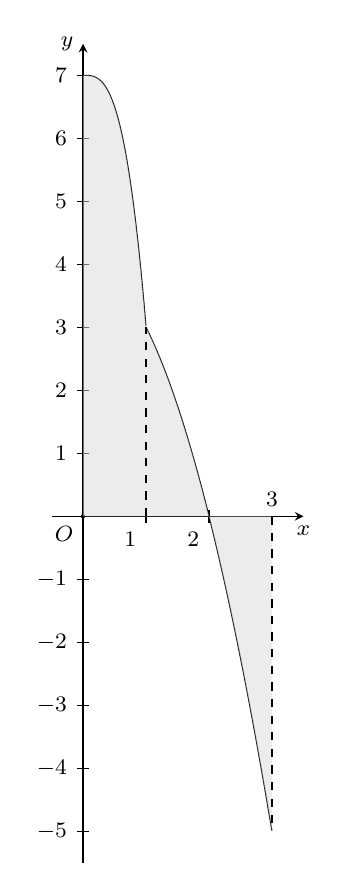
\begin{tikzpicture}[scale=0.8,>=stealth,x=1cm,y=1cm,font=\footnotesize]
				\draw[->] (-0.5,0) -- (3.5,0) node[below] {$x$};
				\draw[->] (0,-5.5) -- (0,7.5) node[left] {$y$};
				\draw (0,0) node[below left] {$O$};
				\foreach \x in {1,2} \draw (\x,0.1) -- (\x,-0.1) node[below left] {$\x$};
				\draw (3,0) node[above]{$3$};
				\fill (0,0) circle (1pt);
				\foreach \y in {-5,-4,-3,-2,-1,1,2,3,4,5,6,7} \draw (0.1,\y) -- (-0.1,\y) node[left] {$\y$};
				\draw[domain=0:1,samples=100] plot (\x,{7-4*(\x)^3});
				\draw[domain=1:3,samples=100] plot (\x,{4-(\x)^2});
				\fill[gray!30,opacity=0.5] (0,0) -- plot[domain=0:1] (\x,{7-4*(\x)^3}) -- (1,0) -- cycle;
				\fill[gray!30,opacity=0.5] (1,0) -- plot[domain=1:2] (\x,{4-(\x)^2}) -- (2,0) -- cycle;
				\fill[gray!30,opacity=0.5] (2,0) -- plot[domain=2:3] (\x,{4-(\x)^2}) -- (3,0) -- cycle;
				\draw[dashed] (1,0) -- (1,3);
				\draw[dashed] (3,0) -- (3,-5);
			\end{tikzpicture}
		}
	}
\end{ex}

\begin{ex}%[2D1H3-6]%[CTST - Lớp 12 - Ôn tập cuối học kì 1 - Đề 5]%[Don Lee]
Khu trò chơi trẻ em Gấu Misa hiện có khách lượng ổn định mỗi ngày là $1\,000$ khách. Mỗi khách vào cổng mua vé giá $40\,000$ đồng. Một cuộc khảo sát cho thấy cứ mỗi lần giảm $2\,000$ đồng giá vé, khu trò chơi có thể có thêm $100$ khách. Để doanh thu thu được là tối đa, khu trò chơi nên bán vé	với giá là bao nhiêu nghìn đồng?
\shortans{$30$}
\loigiai{
Gọi $x$ là số lần giảm $2\,000$ đồng giá vé. Khi đó\\
Giá vé lúc này là $p(x)=40-2x$, với $0<x<20$.\\
Số khách tăng thêm là $100x$. Do đó, tổng số khách là $1\,000+100x$.\\
Hàm doanh thu thu được
\[R(x)=(1\,000+100x)p(x)=(1\,000+100x)(40-2x)=-200x^2+2\,000x+40\,000.\]
Xét hàm $R=R(x)=-200x^2+2\,000x+4\,0000$ trên $(0;20)$.\\
Vì $R=R(x)$ là hàm số bậc hai có hệ số $a<0$, nên $\max R=R(5)$.\\
Vậy doanh thu đạt tối đa khi $x=5$.\\
Điều này tương ứng với $5$ lần giảm $2\,000$, tức là giá vé cần bán ra là $40\,000-5\cdot 2\,000=30\,000$.
}
\end{ex}

\begin{ex}%[2D1H4-3]
	Cho đồ thị hàm số $f(x)=\dfrac{3x+5}{-x+7}$ có tâm đối xứng là $I(a;b)$. Giá trị của biểu thức $B=-4a-b$ là bao nhiêu?
	\shortans[]{-25}
	\loigiai{
		Tập xác định $\mathscr{D}=\mathbb{R}\setminus\{7\}$. \\
		Ta có $\lim \limits_{x\to +\infty}\dfrac{3x+5}{-x+7}=-3$ và $\lim \limits_{x\to -\infty}\dfrac{3x+5}{-x+7}=-3$. \\
		Suy ra đường thẳng $y=-3$ là tiệm cận ngang của đồ thị hàm số. \\
		Lại có $\lim \limits_{x\to 7^+}\dfrac{3x+5}{-x+7}=-\infty$ (do $\lim \limits_{x\to 7^+}(3x+5)=26>0$ và $\lim \limits_{x\to 7^+}(-x+7)=0$; $-x+7<0$, $\forall x>7$). \\
		Tương tự $\lim \limits_{x\to 7^-}\dfrac{3x+5}{-x+7}=+\infty$. \\
		Suy ra đường thẳng $x=7$ là tiệm cận đứng của đồ thị hàm số. \\
		Đồ thị hàm phân thức bậc nhất trên bậc nhất nhận giao điểm của hai đường tiệm cận làm tâm đối xứng nên tọa độ tâm đối xứng là $I(7;-3)$. \\
		Đồng nhất với giả thiết $I(a;b)$, ta được $a=7$ và $b=-3$. \\
		Vậy $B=-4a-b=-4\cdot 7-(-3)=-28+3=-25$.
	}
\end{ex}

\Closesolutionfile{ans}
\indapan{4}{ans/De-TB-Yeu-So-1}
